With a deeper understanding of the historical Jesus, the interpretation of the events that followed his death can change quite dramatically as well.

In the context of an influential royal figure with a large following and with early texts in circulation, the early Christian movement can be seen in a new light.

If we acknowledge that Jesus was framed in Greek and Egyptian royal cult, then Christianity appears from the very beginning as an extension of that tradition.
Jesus did not emerge in a vacuum with completely new ideas.
He was a continuation of the recently fallen Greek empire and inherited a movement that already spanned a major part of Rome.

In this chapter we will try to view the events of the New Testament after Jesus’ death in the light of what we found in previous chapters.
As the Gospel of Matthew closes: πορευθέντες οὖν μαθητεύσατε πάντα τὰ ἔθνη — “Go, therefore, and make disciples of all nations.”

\section{Who were the gentiles?}\label{sec:who-were-the-gentiles}

The word “gentiles” has long been misapplied in the context of the New Testament.
It is almost universally taken to mean “anyone who is not Jewish.”
The confusion comes from the Hebrew word \textit{goyim}, which in many contexts does carry this meaning.
While in the Septuagint, \textit{ethnē} often is used as a translation of \textit{goyim}, it does not show any sign of the same meaning in the context of the New Testament or other Hellenistic works and inscriptions.
The key point missed by most interpreters is that \textit{panta ta ethnē} does not refer to \textit{goyim} or to all peoples universally, but to the nations of the Greek world.
In Hellenistic inscriptions, the phrase “all the nations” (\textit{panta ta ethnē}) is repeatedly used for the \textit{oikoumene}, the civilized world subject to the emperor.
It was imperial language, not global anthropology.
Thus, Matthew’s Great Commission is not an open-ended summons to the Americas or India, but to the Greek-speaking nations of the empire.

Καὶ εὐλογηθήσονται ἐν τῷ σπέρματί σου πάντα τὰ ἔθνη τῆς γῆς — “And in your seed all the nations of the earth shall be blessed” (Gen 22:18 LXX).
This verse is quoted in Galatians 3:8 to argue that “all the nations” were meant to be part of God’s covenant.
Here the nations are not portrayed as outsiders, but as peoples folded into God’s promise.

Βασιλεῖς τῆς γῆς καὶ πάντες λαοὶ, ἄρχοντες καὶ πάντες κριταὶ γῆς… ὕμνος πᾶσι τοῖς ὁσίοις αὐτοῦ, τοῖς υἱοῖς Ἰσραήλ, λαῷ ἐγγίζοντι αὐτῷ — “Kings of the earth and all peoples, rulers and all judges of the earth… a hymn for all His saints, the sons of Israel, a people near to Him” (Ps 148:11, 14 LXX).
The kings and peoples of the earth are included in God’s rule, yet the focus remains on Israel as the center.

The same idiom appears in imperial decrees, for example in the already cited Priene calendar inscription (9 BC), which describes the birthday of Augustus as “gospel for all the nations,” clearly referring to the subjects of the empire rather than to the entire globe.

“All the nations” in these texts does not mean “non-Jews.”
It refers to all peoples under God’s sovereignty, which in a Hellenistic and imperial context meant the nations integrated into the covenantal and political order of the \textit{oikoumene}.
That included Jews as well as Greeks and others within the world of the recently fallen Greek empire.

\section{Are Acts a work of fiction?}\label{sec:are-acts-a-work-of-fiction}

The Acts of the Apostles describes the actions of the apostles after Jesus' ascension and until the revolts against Rome in 66-70 AD .
It follows the travels of Paul and Peter to all the major cities of the former Greek empire, and describes the interactions of the apostles with the church authorities there.
The Acts of the Apostles is often dismissed as a work of fiction.
And indeed, if Acts are read as a history of the spread of a new religion, we already run into major contradictions.
Most notably the churches described in Acts and the epistles appear fully formed, with no indication of how they were established.
There is actually very little in the way of religious conversion in there.
Most places like Athens already believed in one god.
A lot of the speeches in Acts are clearly political speeches, and while there are certainly some religious elements to them, they do not resemble the speeches of a religious missionary.
It is always argued that to be an effective missionary, one must first establish a rapport with the audience, and so describe the local beliefs and then show how the new religion is compatible with them.
And so the definition of God as the omnipotent force behind the universe, who created everything, and who is not confined to a temple, is a perfect fit for the Hellenistic monotheism that was already present in the former Greek empire.
To wit, during the episodes in Ephesus, where there is a strong cult of Artemis, and physical idols, Paul does attack the beliefs directly.
So this looks like praising the modern ideas of Greek faith and denouncing the old ones, not trying to find commonalities between Judaism and the whatever the local beliefs were.

Once we understand more clearly what apostles and churches were, the Acts of the Apostles makes a lot more sense.
For centuries apostles have been emissaries of centralized state and ecclesia is the civic assembly of the city, local government.
These were not religious terms but administrative ones.
We have well-developed councils, bishops, deacons and treasuries.
This makes absolutely no sense if we assume this is a formation of a new church with a handful of members.
It makes a lot of sense if we remember all of this already existed as part of the Greek civic order, and the apostles were simply trying to maintain the existing order under a new reality of Roman rule.
In that light the Acts of the Apostles is a record of trying to maintain the Greek civic order under a new reality of Roman rule.
There are many references to acts of recommendation, letters of introduction, confiding common law between the ecclesia of different cities, and numerous references to newly appointed officials.
After the conquest and the rebellions, the texts were indeed altered to account for a failed rebellion rather that a failed prophecy of the end of the world.

Like we see clear additions in the gospels that are often dated to 70 AD or shortly after, we can suspect that the Acts of the Apostles were written at the time of the edits.
We are looking here at the second generation of Greeks and Jews under direct and harsh Roman rule coming to terms with the reality of failed rebellions.

\subsection{What is quite striking is that Paul and others write to so many different churches over the short period of time.}\label{subsec:what-is-quite-striking-is-that-paul-and-others-write-to-so-many-different-churches-over-the-short-period-of-time.}

There is a major challenge for the traditional timeline of the apostles establishing so many churches in such a short period of time.
These churches would have to all be established, grow, keep up to date with the fastly shifting theology, and then do nearly nothing for the next 100 years.
These churches immediately showed up in every single major city in the former Greek empire, and no churches showed up anywhere else.
All of the correspondence and scripture was written in Greek, and no other languages.
It is important to point out that Greek was absolutely not the lingua franca in any part of the Roman empire that was not recently part of the Greek empire.
The lingua franca of the Roman empire was Latin, and that was the only language that was used in the administration and the primary language used by the authors.
If the apostles were to establish churches everywhere in the Roman empire, and not just in the former Greek empire, then we would have had the epistles to the extremely prominent cities of Mediolanum, Lutetia, Aquilea, Lugdunum, Memphis, and Londinium.
The truth is that no matter how we model the growth of the early church, it is not possible to explain the the patterns we observe.
And then for the next 100 years do not add any new churches.

Even more striking is the total absence of Aramaic or Hebrew letters.
If the apostles’ mission were Jewish in nature, at least some correspondence would survive in the languages of Judea.
Instead, all the letters are in Greek, to Greek assemblies, proving that the movement was imperial and Hellenistic at its core.

\subsection{Paul’s letters as state correspondence.}\label{subsec:pauls-letters-as-state-correspondence.}

The epistles resemble circular letters of the Hellenistic and Roman administrations.
They are addressed to \textit{ekklesiai}, the same word used for political assemblies of citizens in Greek cities.
Paul is not writing to small house cults, but to recognized civic assemblies under a higher king.
This gives the Pauline corpus the character of imperial decrees rather than private exhortations.

There were essentially no prominent cities in the former Greek empire that were not mentioned in the Acts and the epistles:
These letters name couriers and order public reading and inter-city circulation, exactly as civic circulars do (cf.\ the exchange instructions for neighboring assemblies).
They carry greetings from co-workers the way chancery letters list co-signatories.
They include directives, adjudications, financial instructions, muster language, and discipline protocols.
They function as decrees to be read \emph{in assembly} and enacted across a network of poleis.
Nothing here looks like a private house cult.
Everything reads like state correspondence to the existing \textit{ekklesiai} of the Greek cities, continuing their business under the banner of the \textit{Christos}.

\subsection{Ekklesia — the civic assembly continued}\label{subsec:ekklesia-the-civic-assembly-continued}

The word ἐκκλησία did not name a new religious club.
It was the same civic assembly that governed the Greek city before the Roman conquest.
It was the same sovereign body of citizens that passed laws, heard proclamations, and received official dispatches.
After conquest the population and magistrates sought continuity, not reinvention.
They kept their assemblies, their procedures, and their language.
Only the allegiance changed.
The assembly now recognized the rightful \textit{Christos} instead of Rome.
This is why all the correspondence is in Greek.
This is why the addressees are the historic poleis of the Greek world.
Paul is not inventing a “church.”
He is addressing the standing political assemblies of the Greek cities as they realign themselves to the true king.

As established in Chapter 2, the ecclesia was not merely a religious gathering but the governing body of the Greek city, complete with civic offices, governance procedures, and social functions.
The epistles confirm this institutional continuity at every level.

\subsubsection{Diakonoi and episkopoi: civic offices already functioning}\label{subsubsec:diakonoi-and-episkopoi-civic-offices-already-functioning}

Paul's earliest letters do not introduce new offices; they address existing ones.
Philippians 1:1 (written c.~60--62 AD) opens: "Paul and Timothy, servants of Christ Jesus, to all the saints in Christ Jesus who are at Philippi, with the \textit{episkopoi} and \textit{diakonoi}" (overseers and deacons).
This is a standard civic salutation.
Paul does not explain what these offices are because the Philippian assembly already knows: they are the same officials who managed the civic assembly before.

Romans 16:1 (c.~57 AD) commends Phoebe as a \textit{diakonos} of the assembly at Cenchreae.
She is not a volunteer; she holds an administrative office, the same office documented in Greek civic assemblies and temple complexes for centuries.
Epigraphic evidence makes this continuity concrete rather than rhetorical.
The Erythrai decree (AIO 296, fifth century BC) names \textit{episkopoi} as civic magistrates who ``allot and install the Council,'' establishing the title within formal political administration.
A statue base on the Athenian Acropolis (IG II² 3464) honours Syeris, \textit{diakonos} of the priestess Lysimache, showing the office embedded in the state cult of Athena Polias.
Jewish diaspora inscriptions from Asia Minor list \textit{gerousiarch}, \textit{grammateus}, and \textit{diakonos} together as standard communal offices, demonstrating that \textit{diakonoi} belonged to the wider Hellenistic administrative vocabulary, not a Christian invention.
Inscriptions from Termessos and Mylasa attest an \textit{ekklesia kyria} still active under Roman rule, proving that the civic assembly remained a functioning institution in the first century.
Later material from Messene shows the same trajectory: a classical assembly hall remodeled in the fourth century by \textit{episkopos} Theodoulos, whose donor inscription lies in the mosaic floor, marking the literal takeover of civic space by Christian officers.
The Pastoral Epistles (1 Timothy 3:1--13) later codify qualifications for \textit{episkopoi} and \textit{diakonoi}, but these read as regulations for \emph{existing} offices, not as the invention of new ones.
The complexity and specificity---managing households, financial integrity, temperance---presume an established administrative role, not a blank slate.

Chapter 2 demonstrated that \textit{diakonoi} managed communal meals in Greek assemblies, assisted in temple rites, and served in Hellenistic cults (including Isis and Serapis).
Paul's letters confirm these exact functions: \textit{diakonoi} handle financial collections (2 Corinthians 8--9), coordinate logistics, and serve at communal meals (1 Corinthians 11).
These are civic stewards continuing their institutional role under a new sovereign.

\subsubsection{Civic governance procedures in the epistles}\label{subsubsec:civic-governance-procedures-in-the-epistles}

The epistles employ the full vocabulary of Greek civic administration.
Philippians 3:20 declares "our \textit{politeuma} is in heaven."
\textit{Politeuma} is not "citizenship" in the abstract; it is civic enrollment, the register of a political community with jurisdiction and legal standing.
Paul is asserting that the Philippian assembly's true civic authority derives from the heavenly king, not from Rome.

Romans 13:1 and Colossians 1:16 use \textit{archai} and \textit{exousiai}---magistracies and jurisdictions---the same terms employed in civic decrees and imperial administration.
These are not mystical concepts; they are constitutional offices.
Paul treats them as such, mapping the believers into a bureaucratic order under Christ as supreme magistrate.

Financial administration appears immediately and in detail.
1 Corinthians 16:1--4 instructs the assembly to organize a collection, appoint delegates, and transfer funds to Jerusalem.
2 Corinthians 8--9 describes inter-city financial coordination, accountability measures, and competitive giving between assemblies.
This is civic governance, not personal charity.
It presumes treasuries, ledgers, and auditing procedures---the infrastructure of the Greek assembly.

Public reading protocols mirror civic procedure.
1 Thessalonians 5:27: "I charge you by the Lord to have this letter read to all the brothers."
Colossians 4:16: "When this letter has been read among you, have it also read in the assembly of the Laodiceans, and see that you also read the letter from Laodicea."
These are the circulation and public reading protocols of official civic circulars, not private correspondence.
Paul is issuing decrees to be proclaimed in assembly and exchanged between cities, exactly as a Greek magistrate or royal emissary would.

\subsubsection{Sociological continuity: status, factions, and the civic catwalk}\label{subsubsec:sociological-continuity-status-factions-and-the-civic-catwalk}

Chapter 2 demonstrated that the Greek ecclesia served a sociological function: it was the primary venue for status display, where families dressed their best, displayed wealth, and enacted social hierarchy.
Ancient sources---Aristophanes, Demosthenes, Athenian scholia---mockingly describe "overdressed youths" and citizens "showing off garments and jewelry" at civic gatherings.
The epistles confirm this behavior continued without interruption.

1 Corinthians 11:17--34 describes the communal meal at Corinth: the rich arrive early, consume the food and wine, and leave the poor with nothing.
Some are hungry; others are drunk.
Paul condemns this not as a new problem but as a violation of the assembly's purpose.
The theological dispute is riding on sociological rails inherited from the civic assembly.
The assembly has become a venue for economic competition and status performance, exactly as it functioned in the Greek civic context.

1 Corinthians 11:2--16 addresses head coverings and appearance during assembly.
This is not about piety; it is about public presentation.
The debate over veiling, hairstyles, and gendered appearance makes sense only in a context where the assembly functions as a civic stage, where participants are seen and judged.

James 2:1--7 condemns favoritism toward the rich: "Suppose a man comes into your assembly wearing a gold ring and fine clothes, and a poor man in shabby clothes also comes in.
If you show special attention to the man wearing fine clothes... have you not discriminated?"
This scenario presumes the assembly is a place where economic status is displayed through clothing and jewelry, where social comparison is constant, and where deference to wealth is a live temptation.
This is the Greek civic assembly in operation.
Notably, gold rings and reserved seating by status are Greek civic markers, not distinctively Jewish; first-century diaspora synagogues themselves adopted Greek governance structures (archons, gerousia, grammateis), functioning as polis-style civic groups within the Hellenistic world.

1 Corinthians 1:10--17 describes factions: "I follow Paul," "I follow Apollos," "I follow Cephas."
This is not only sectarian theology but also civic faction politics.
Greek assemblies were notorious for splits along patronage lines, with rival orators attracting competing blocs.
Paul's Corinthian assembly exhibits the same dynamic, because it \emph{is} the same institution, operating under the same social logic.

The assemblies did not need to \emph{learn} how to have factions, manage money, read decrees aloud, display status, or appoint officials.
They already knew, because they had been doing it for centuries.

\subsubsection{Institutional complexity appears instantly: not evolution but continuation}\label{subsubsec:institutional-complexity-appears-instantly-not-evolution-but-continuation}

Traditional models assume early Christianity began as a handful of believers in house meetings and gradually developed institutional structures over generations.
The epistles refute this.
Moreover, references to house meetings appear in \emph{later} epistles (Romans 16:5, Philemon 1:2, Colossians 4:15), suggesting that the shift to household gatherings reflects increasing Roman surveillance rather than the original institutional form.
As Roman rule strengthened and political assemblies came under closer scrutiny, some meetings moved to more covert locations.
This is evidence \emph{for} political continuity---assemblies forced underground by imperial crackdown---not evidence against it.
The behavior described remains empirically civic: factions, financial systems, status display, and inter-city coordination.
1 Corinthians, written c.~54--55 AD---only twenty to twenty-five years after Jesus' death---already describes:
\begin{itemize}
    \item Multiple factions with competing leaders and theological positions
    \item Established liturgical practices (baptism formulas, Eucharist protocols, creedal recitations)
    \item Complex financial systems with collection, delegation, and inter-city coordination
    \item Offices with defined qualifications and responsibilities
    \item Discipline procedures including exclusion and reinstatement
    \item Legal arbitration within the assembly (1 Corinthians 6:1--8)
    \item Public reading and circulation of authoritative letters
\end{itemize}

1 Corinthians is written barely twenty to twenty-five years after Jesus' death, yet it presupposes an assembly that already knows how to handle factions, liturgy, finance, discipline, and inter-city coordination.
To explain this as something invented from scratch in a single generation requires us to posit the fastest institutionalization of any religious movement we know from antiquity.
It is far more economical to recognize that these were not naïve "house churches" discovering governance for the first time, but long-standing civic assemblies and association-forms being re-aligned: the same officials, the same procedures, the same social logic---now acting under a different king.

The geographic evidence supports this institutional continuity model decisively.
The next Christian city to appear \emph{after} the New Testament's Greek world is Carthage, and it appears in the late second century (c.~180--200 AD, attested in the Scillitan Martyrs and Tertullian).
This is the first Christian city that is not part of the Pauline network and not mentioned in the New Testament.
If Christianity had spread through missionary preaching, Carthage---a major port city with established trade routes to Rome and the eastern Mediterranean---would have been Christian by 60--80 AD.
Instead it appears 120--140 years later.
Even Alexandria---the second largest city in the empire---enters the Christian record only around 189--200 AD, with Demetrius and Clement of Alexandria.
No first-century or early second-century source mentions an Alexandrian church at all.

This is not merely absence of evidence; it is evidence of absence.
Numerous early Christian writings survive from the first half of the second century---1 Clement (c.~96 AD), Ignatius of Antioch (c.~110 AD), the Didache (c.~80--120 AD), the Shepherd of Hermas (c.~90--140 AD), Papias of Hierapolis (c.~120 AD), Quadratus (c.~125 AD), Aristides (c.~125--135 AD), Polycarp (mid-second century), and Hegesippus (c.~160--180 AD, who traveled the empire documenting Christian communities)---and not one mentions any Western location at all.
These authors actively list churches, send letters, and reference Christian communities across the eastern Mediterranean, yet they show zero awareness of churches in Gaul, Spain, North Africa, Germania, or Britain.
Even Clement of Rome and the Shepherd of Hermas, both written \emph{in} Rome, mention no Western Christian communities beyond Rome itself.
No biological, sociological, or political model produces instant global spread followed by 120 years of total silence in the most connected regions of the empire.
This is not slow growth; it is no growth.
The pattern is definitive: where Greek civic assemblies existed, Christianity appears instantly in the first century.
Where they did not exist, Christianity appears centuries later.

The continuity here is structural and sociological, not theological.
The question is not what Christians believed, but what institutional forms they used.
This reading does not claim \emph{pure} continuation; Paul's assemblies are hybrid institutions where civic assembly, diaspora synagogue, and voluntary association logics overlap.
Diaspora synagogues themselves functioned with civic-administrative features---officers, treasurers, communal courts---making them compatible with the civic \emph{ekklesia} frame.
Recognizing hybridity avoids reductionism: the continuity argument concerns administrative and sociological structures, not theological content.
But for the Greek-speaking cities Paul addresses, the \emph{ekklesia} term and the observed behaviors map most strongly onto civic practice, supported by scholars such as Young-Ho Park (\emph{Paul's Ekklesia as a Civic Assembly}, 2015), Philip Esler (2021), and George van Kooten, who have independently argued that early Christian assemblies must be understood in the context of continuing political institutions rather than as purely novel religious formations.

Papyrological evidence confirms that these assemblies were visible to Roman administration as corporate bodies.
P.Oxy.~8.1138 records a money-tax paid ``on behalf of the \textit{ekklesia},'' phrased in the same bureaucratic formula used for professional guilds and civic associations.
P.Oxy.~33.2673, from the Great Persecution, inventories church property with the standard confiscation language of imperial edicts, listing books, vessels, and assets exactly as the state recorded the goods of any other registered institution.
These documents prove that Roman officials treated the \textit{ekklesia} as a corporate actor, capable of holding property, receiving assessments, and being targeted by administrative sanctions.
They show continuity not of beliefs but of institutional form: a body with officers, treasurers, buildings, and legal presence within provincial bureaucracy.

At this point we must be explicit about what the evidence can and cannot demonstrate.
We do not yet possess an inscription that declares ``the \textit{ekklesia} of Ephesus, which once sacrificed to Artemis, now recognizes Christos.''
What we do have is the uninterrupted appearance of civic titles, civic procedures, civic building usage, and civic bureaucratic visibility under the new allegiance to Christ.
The pattern shows structures that do not dissolve and reconstitute themselves but simply shift their sovereign referent.
The transformation lies in political loyalty rather than institutional architecture.
A polis assembly that once owed its dignity to the imperial cult could redirect its honor language, its oaths, and its benefaction system toward a different king without altering its internal mechanics.
Offices such as \textit{episkopos} and \textit{diakonos} continue because they already carried administrative meaning in the civic and cultic world.
Communal meals, treasuries, and gatherings continue because these practices belong to the sociological function of assemblies, not to any single theology.
Paul's communities read as assemblies whose rituals, hierarchy, and administrative logic remain familiar, while the central object of loyalty---Christ instead of Caesar---constitutes the real rupture.
The evidence therefore points to political realignment rather than institutional reinvention.
Christianity enters the civic field by redirecting allegiance inside existing structures, not by creating an alternative universe of religious associations.
The \textit{ecclesiae} of the first century are best understood as assemblies that changed their king, not their form.

\subsubsection{Geographic evidence: exhaustive mapping reveals a political boundary, not missionary diffusion}

The power of this institutional continuity argument becomes undeniable when we methodically map \emph{every} city mentioned in Acts and the Epistles.
This is not cherry-picking; it is exhaustive cataloging.
When we plot all named locations---every city where Paul preached, where assemblies met, where letters were sent---a striking pattern emerges: they align almost perfectly with the former territories of the Greek empire (Ptolemaic Egypt, Seleucid Syria, Macedonian Greece, and Hellenistic Asia Minor).
There were essentially no prominent cities in the former Greek empire that were not mentioned in the Acts and the Epistles, and conversely, there were essentially no cities mentioned in the New Testament that were not part of this Greek-speaking world.
The geographic distribution is not random missionary expansion; it is a political map:

Judea and Surrounding Regions: \textbar{} Region \textbar{} City \textbar{} Reference(s) \textbar{} Notes \textbar{} \textbar---------------------------\textbar--------------\textbar---------------------------------------\textbar-----------------------------------------------------------------------\textbar{} \textbar{} Judea and Surrounding Regions \textbar{} Jerusalem \textbar{} Acts 1:4, 2:5, 8:1 \textbar{} Center of the early Christian movement and where Pentecost occurred.
\textbar{} \textbar{} \textbar{} Bethany \textbar{} Acts 1:12 \textbar{} Near Jerusalem, where Jesus ascended to heaven.
\textbar{} \textbar{} \textbar{} Joppa \textbar{} Acts 9:36 \textbar{} A port city where Peter stayed and raised Tabitha from the dead.
\textbar{} \textbar{} \textbar{} Caesarea \textbar{} Acts 8:40, 10:1 \textbar{} Where Philip preached and where Cornelius, a Gentile, was baptized by Peter.
\textbar{} \textbar{} \textbar{} Antioch \textbar{} Acts 11:19 \textbar{} A key city for early Christian missions and where followers of Jesus were first called Christians.
\textbar{} \textbar{} \textbar{} Nazareth \textbar{} Acts 2:22 \textbar{} Hometown of Jesus, mentioned in the sermon at Pentecost.
\textbar{} \textbar{} Asia Minor (Modern-day Turkey) \textbar{} Tarsus \textbar{} Acts 9:11 \textbar{} The birthplace of Paul (Saul).
\textbar{} \textbar{} \textbar{} Lystra \textbar{} Acts 14:6 \textbar{} Where Paul healed a crippled man and was nearly stoned.
\textbar{} \textbar{} \textbar{} Derbe \textbar{} Acts 14:6 \textbar{} Where Paul and Barnabas preached and made many disciples.
\textbar{} \textbar{} \textbar{} Iconium \textbar{} Acts 14:1 \textbar{} Where Paul preached and faced opposition from the local Jewish authorities.
\textbar{} \textbar{} \textbar{} Ephesus \textbar{} Acts 18:19 \textbar{} A major city in Asia Minor where Paul spent a significant amount of time preaching and establishing the church.
\textbar{} \textbar{} \textbar{} Miletus \textbar{} Acts 20:15 \textbar{} Where Paul met with the Ephesian elders on his way to Jerusalem.
\textbar{} \textbar{} \textbar{} Smyrna, Pergamum, Thyatira, Sardis, Philadelphia, Laodicea \textbar{} Revelation letters \textbar{} Acts doesn't mention directly but likely influenced early Christian activity.
\textbar{} \textbar{} Greece \textbar{} Philippi \textbar{} Acts 16:12 \textbar{} Where Paul and Silas were imprisoned and where the first European Christian church was founded.
\textbar{} \textbar{} \textbar{} Thessalonica \textbar{} Acts 17:1 \textbar{} A major city where Paul preached and faced opposition.
\textbar{} \textbar{} \textbar{} Berea \textbar{} Acts 17:10 \textbar{} Where Paul went after Thessalonica and found the Bereans to be more receptive to the gospel.
\textbar{} \textbar{} \textbar{} Athens \textbar{} Acts 17:16 \textbar{} Where Paul preached on Mars Hill and engaged with philosophers about the ``unknown god.'' \textbar{} \textbar{} \textbar{} Corinth \textbar{} Acts 18:1 \textbar{} Where Paul stayed and established a Christian community, and where he later wrote 1 and 2 Corinthians.
\textbar{} \textbar{} Macedonia and the Surrounding Areas \textbar{} Neapolis \textbar{} Acts 16:11 \textbar{} Port city in Macedonia, where Paul and his companions arrived after sailing from Troas.
\textbar{} \textbar{} \textbar{} Philippi \textbar{} Acts 16:12 \textbar{} Mentioned earlier in Greece.
\textbar{} \textbar{} Egypt \textbar{} Alexandria \textbar{} Acts 6:9, 18:24 \textbar{} Apollos was from here; a major Jewish and early Christian hub.
\textbar{} \textbar{} Libya (North Africa) \textbar{} Cyrene \textbar{} Acts 2:10, 11:20 \textbar{} Home of Simon of Cyrene; some early Christians were from here.
\textbar{} \textbar{} Italy and Rome \textbar{} Puteoli \textbar{} Acts 28:13 \textbar{} Port city in Italy where Paul arrived after sailing from Malta.
\textbar{} \textbar{} \textbar{} Rome \textbar{} Acts 28:16 \textbar{} Where Paul was taken as a prisoner and spent two years under house arrest.
\textbar{} \textbar{} Other Notable Cities \textbar{} Cyprus \textbar{} Acts 13:4 \textbar{} Where Paul and Barnabas first traveled for missionary work.
\textbar{} \textbar{} \textbar{} Salamis \textbar{} Acts 13:5 \textbar{} A city in Cyprus where Paul preached.
\textbar{} \textbar{} \textbar{} Paphos \textbar{} Acts 13:6 \textbar{} A city in Cyprus where Paul encountered the sorcerer Elymas.
\textbar{} \textbar{} \textbar{} Patara \textbar{} Acts 21:1 \textbar{} A port city in Lycia where Paul caught a ship to Phoenicia.
\textbar{} \textbar{} \textbar{} Tyre \textbar{} Acts 21:3 \textbar{} A city in Phoenicia where Paul stopped to meet the disciples.
\textbar{}

Regions and Cities in the Epistles:

\begin{longtable}[]{@{}p{0.15\linewidth} p{0.15\linewidth} p{0.7\linewidth}@{}}
    \toprule\noalign{}
    \begin{minipage}[b]{\linewidth}\raggedright
    Location
    \end{minipage} & \begin{minipage}[b]{\linewidth}\raggedright
    Mentioned In
    \end{minipage} & \begin{minipage}[b]{0.7\linewidth}\raggedright
    References
    \end{minipage} \\
    \midrule
    \endhead
    \bottomrule
    \endlastfoot
    Rome & Acts, Romans, Philippians, 2 Timothy & Acts 28, Romans 1:7, 1:15, Philippians 1:13, 2 Timothy 4:16-17 \\
    Corinth & Acts, 1 Corinthians, 2 Corinthians & 1 Corinthians 1:2, 2 Corinthians 1:1 \\
    Ephesus & Acts, Ephesians & Ephesians 1:1 \\
    Galatia & Galatians & Galatians 1:2 \\
    Philippi & Acts, Philippians & Philippians 1:1 \\
    Thessalonica & 1 Thessalonians, 2 Thessalonians & 1 Thessalonians 1:1, 2 Thessalonians 1:1 \\
    Colossae & Colossians & Colossians 1:2 \\
    Laodicea & Colossians, Revelation & Colossians 4:13-16, Revelation 3:14-22 \\
    Crete & Titus & Titus 1:5 \\
    Cyprus & Galatians & Galatians 4:13 \\
    Pontus, Galatia, Cappadocia, Asia, Bithynia & 1 Peter & 1 Peter 1:1 \\
    Macedonia & 2 Corinthians, Philippians & 2 Corinthians 8:1, Philippians 4:15 \\
    Miletus & 2 Timothy & 2 Timothy 4:20 \\
    Antioch & Acts, Galatians, 1 Corinthians & Galatians 2:11, 1 Corinthians 9:6 \\
    Tarsus & Acts, 2 Corinthians & Acts 9:11, 2 Corinthians 11:22 \\
    Syria & 1 Corinthians, Galatians, 2 Corinthians & 1 Corinthians 16:3, Galatians 1:21, 2 Corinthians 11:9 \\
    Asia & 1 Corinthians, 2 Corinthians, Revelation & 1 Corinthians 16:19, 2 Corinthians 1:8 \\
    Troas & Acts, 2 Timothy & Acts 20:6, 2 Timothy 4:13 \\
    Berea & Acts, 1 Thessalonians & Acts 17:10, 1 Thessalonians 1:7 \\
    Paphos & Acts, Titus & Titus 1:5 \\
    Puteoli & Romans & Romans 16:3-4 \\
\end{longtable}

It is important to actually visualize the locations mentioned in the Acts and the epistles to see the striking pattern of the locations mentioned in the Acts and the epistles being the same as the most significant Greek speaking cities.

\begin{figure}[ht]
    \centering
    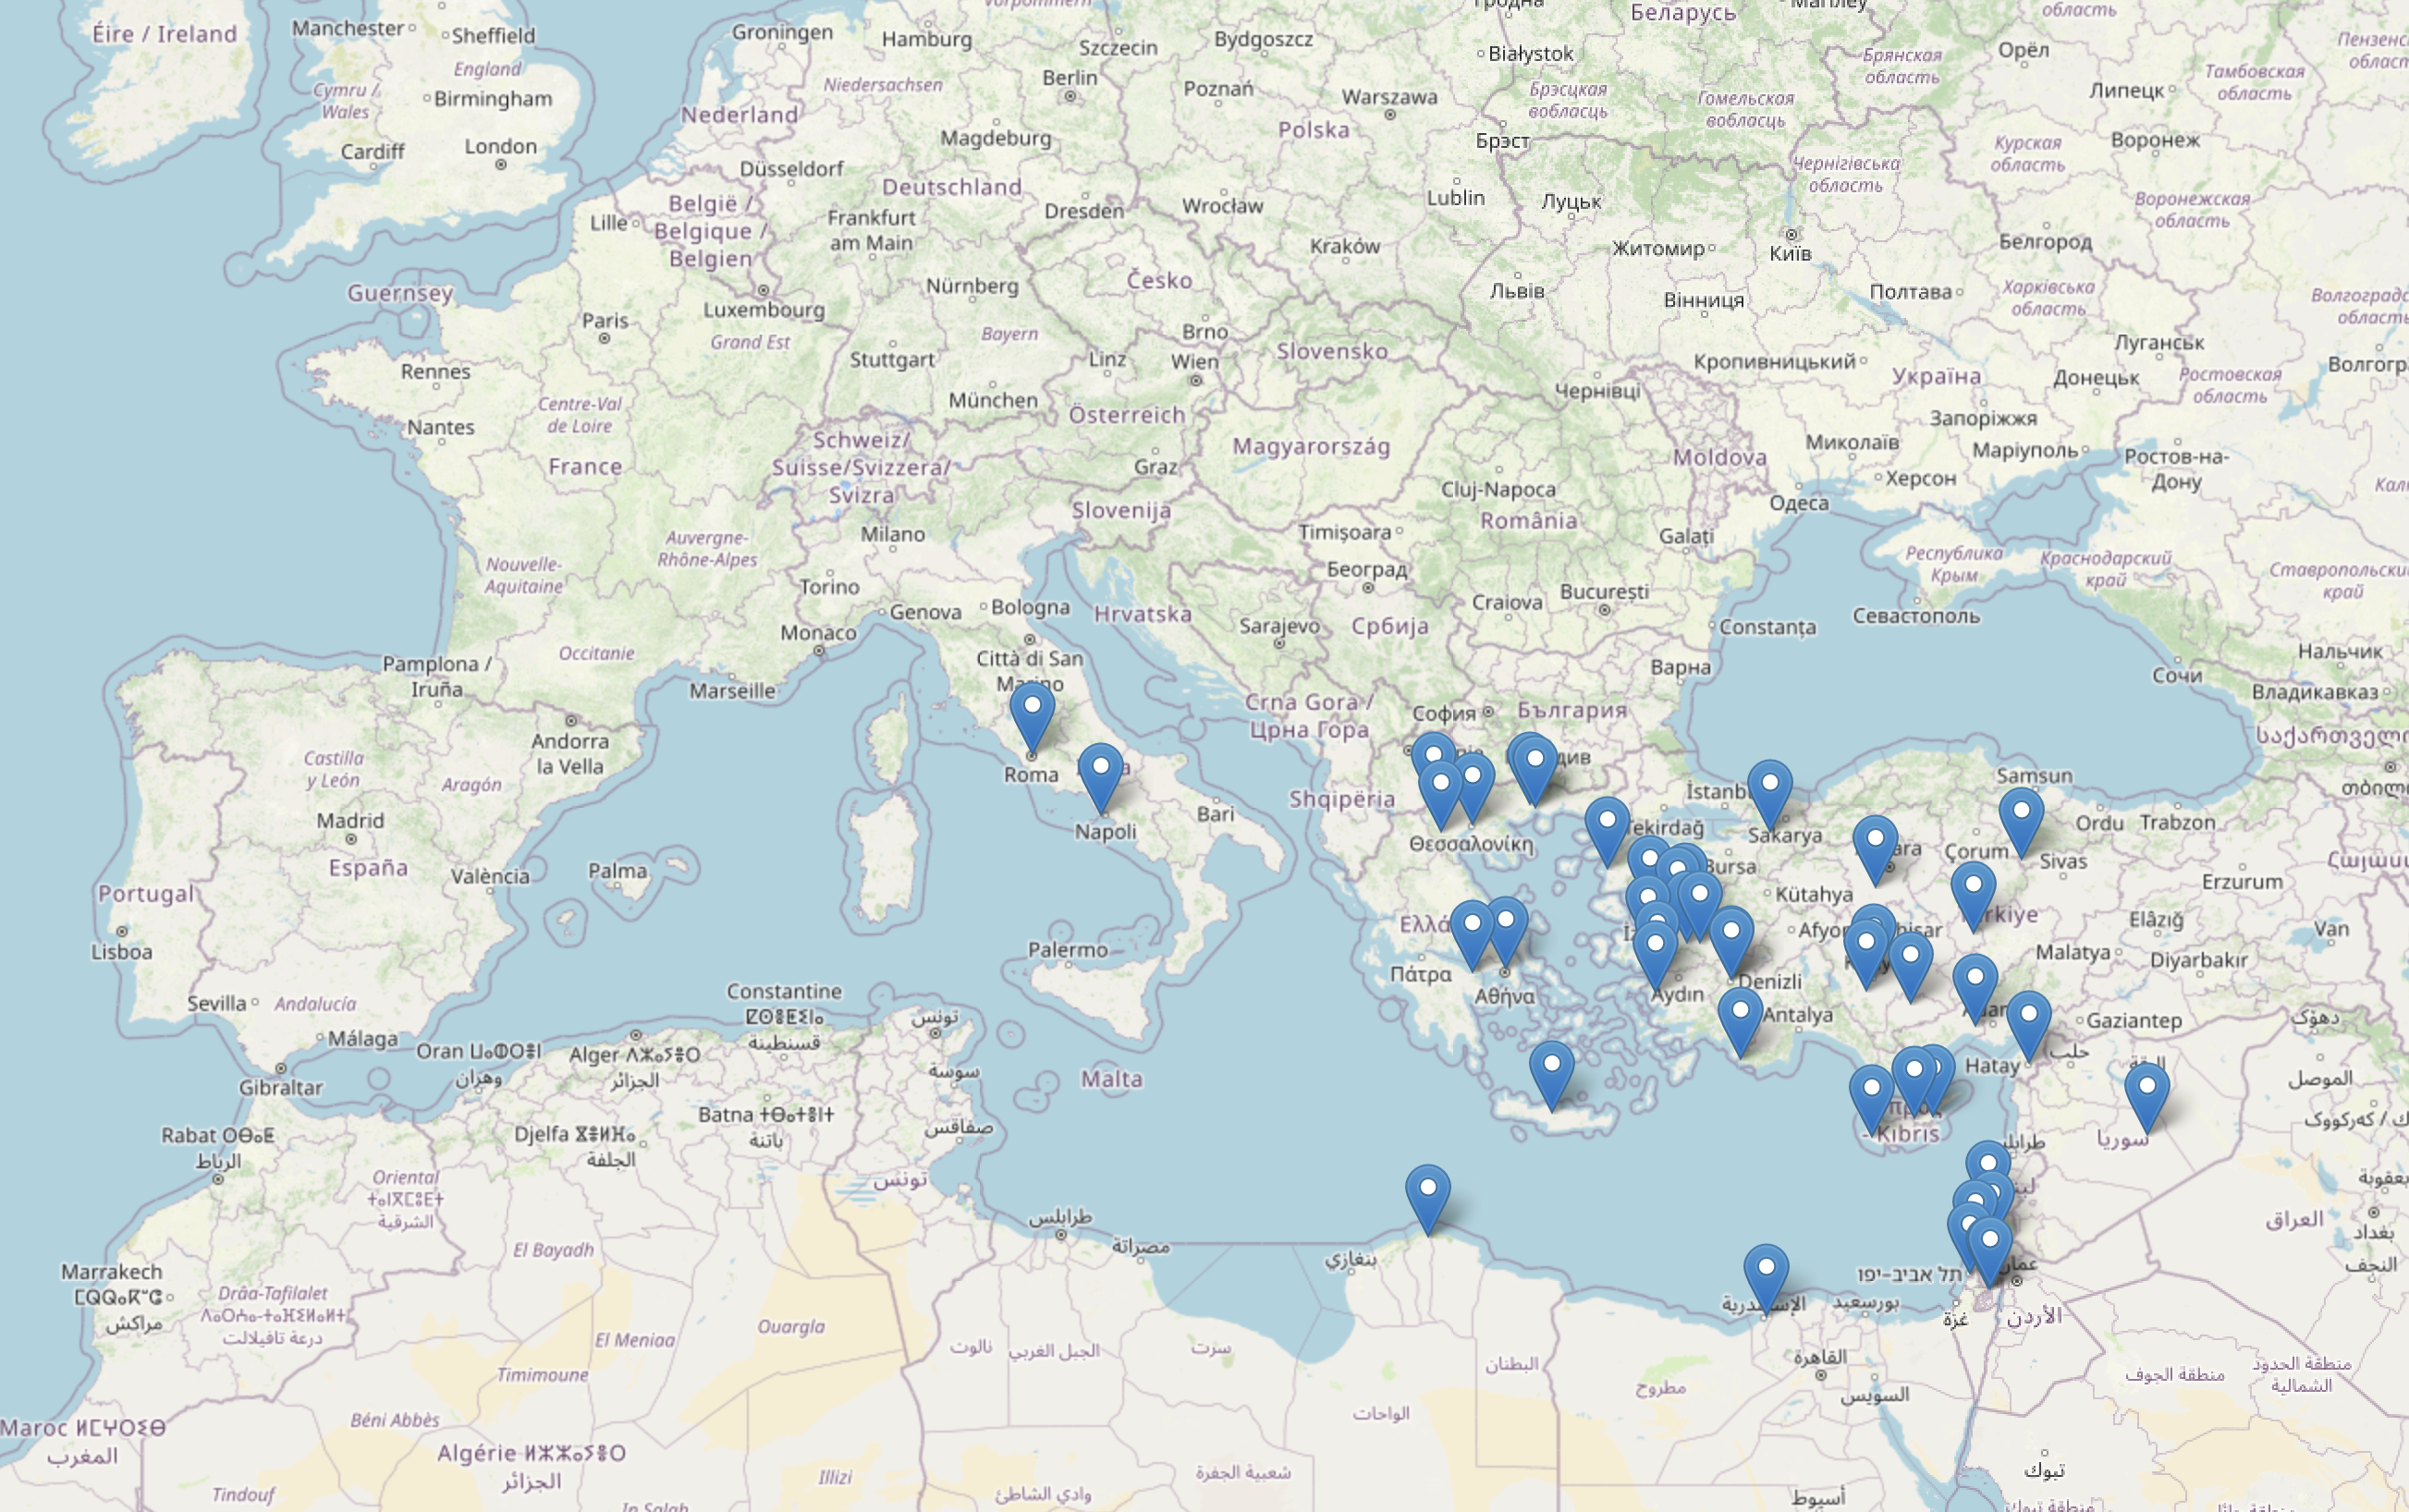
\includegraphics[width=\textwidth, keepaspectratio]{assets/locations_map}
    \caption{Map of all the locations mentioned in the Acts and the epistles.}
    \label{fig:figure}
\end{figure}

For those geographically inclined you can spot the near perfect correlation with the borders of Eastern Roman Empire.
Of note is the trip to Rome, which was substantially different in nature to the other trips.
\href{https://en.wikipedia.org/wiki/Byzantine_Empire_under_the_Theodosian_dynasty\#/media/File:4KTHEODOSIAN.png}{Rome Map}

\subsection{The striking statistics of the cities mentioned in the Acts and the epistles are that they are all in the former Greek empire, and not one mention of a city in the Roman empire that was not part of the former Greek empire.}\label{subsec:the-striking-statistics-of-the-cities-mentioned-in-the-acts-and-the-epistles-are-that-they-are-all-in-the-former-greek-empire-and-not-one-mention-of-a-city-in-the-roman-empire-that-was-not-part-of-the-former-greek-empire.}

This fact makes any theory that deems Christianity as a religious and not a political movement immediately highly implausible.

\subsection{Minimal resistance to the acceptance of the new religion.}\label{subsec:minimal-resistance-to-the-acceptance-of-the-new-religion.}

The new religion was accepted by the masses in the former Greek empire, and not a single mention of any resistance to the new religion from the Greeks themselves.
The only real opposition comes from the Temple authorities in Jerusalem.
This is consistent with Christianity being a continuation of Greek imperial philosophy, which the Hellenized population already accepted.

\subsection{Even though the religion was so successful at converting the masses, it still had all the conspiratorial parts to it.}\label{subsec:even-though-the-religion-was-so-successful-at-converting-the-masses-it-still-had-all-the-conspiratorial-parts-to-it.}

Early Christians used secret symbols to identify each other, they frequently met in secret, often at night in the catacombs.
This is not unlike the initiation practices of other imperial soldier cults such as Mithras.
The Pauline language of ``soldiers of Christ'' fits this conspiratorial military model.

\subsection{Christianity much more prosecuted than any other religion in the Roman empire.}\label{subsec:christianity-much-more-prosecuted-than-any-other-religion-in-the-roman-empire.}

The Roman empire was very tolerant of other religions, and the only time they would prosecute a religion was if it was a threat to the empire.
Christians were persecuted not for worshipping a strange god, but for refusing the Roman emperor cult while insisting that only their Christ was king.

First of all we must acknowledge that the most broadly known source of early Christian prosecution, the Nero accusation of Christians starting the Great Fire of Rome, is now widely discredited as a fabrication.
Tacitus in his work talks about Chrestos that is  a very common name and almost certainly not a reference to Jesus.
When first writing about the Christians, Tacitus, fifty years after the events is not familiar with the group.
The same can be said about Pliny the Younger, who in his letter to Trajan is not familiar with the Christians.
If Christians were blamed for the largest disaster in the lives of both Tacitus and Pliny, it would be inconceivable that they would not know about it.

At the same time, Peter was executed in Rome by crucifixion, and Paul was executed by beheading.
Like with Jesus, crucifixion was reserved for crimes against the state, sedition, and treason.
As Paul was a Roman citizen, he would have been beheaded for the same crimes.
If there was no organized persecution of Christians, it is hard to explain why both Peter and Paul were executed in such a manner.

\subsection{The phrase ``soldiers of Christ'' is not used explicitly in the Gospels, but it appears prominently in the Pauline Epistles.}\label{subsec:the-phrase-soldiers-of-christ-is-not-used-explicitly-in-the-gospels-but-it-appears-prominently-in-the-pauline-epistles-particularly-in-the-context-of-the-christian-life-being-compared-to-a-military-struggle-or-a-spiritual-battle.}

The metaphor emphasizes loyalty, discipline, and readiness for conflict under a divine king.
It reflects the military cultic environment of the empire, not a rural Jewish sect.

\section{The early dating of the gospels can make the letters of Paul more plausible as it seems Paul already has the knowledge of at least one of the gospels and the acts.}\label{sec:the-early-dating-of-the-gospels-can-make-the-letters-of-paul-more-plausible-as-it-seems-paul-already-has-the-knowledge-of-at-least-one-of-the-gospels-and-the-acts.}

Many scholars dispute the existence of Paul based on the striking contradiction in mainstream scholarship that authors of Pauline epistles seem to have the knowledge of the gospels and the acts, and yet the gospels and the acts are unanimously dated to be written after the Pauline epistles.
In here the existence of Paul can once more be reconsidered if we acknowledge the early dating of the gospels and the gospel of John in being written by an eyewitness of Jesus's life.

\subsection{Paul barely mentions the life of Jesus, and almost never quotes him.}\label{subsec:paul-barely-mentions-the-life-of-jesus-and-almost-never-quotes-him.}

It is frequently claimed that Paul's religion is not the religion of Jesus, but the religion about Jesus.
There is a shocking lack of references to any of the teachings of Jesus, the Jewish law, and any of the events surrounding Jesus's life and death.
So we may go one step further.
It is a religion focusing on restoring the kingdom of God by resurrecting the office of the Christos, the rightful king of the kingdom of God.
And so to Paul and all the early Christians, it was all about resurrecting a Christ, not teachings of the particular Jesus Christ.
The idea that God will once again send a king that will restore the Greek empire, the kingdom of God, headed by Christos, the rightful earthly king of the kingdom of God.

\subsection{7a.
Paul fuses army and court: enlistment under the Christ and absorption into his imperial bureaucracy.}\label{subsec:pau-fuses-army-and-court-enlistment-under-the-christ-and-absorption-into-his-imperial-bureaucracy.}

This is not angelic poetry; it is administrative vocabulary.
Paul lists “thrones, dominions, principalities, and authorities” (\emph{thronoi, kyriotētes, archai, exousiai}) as if reading out a court register (Col 1:16; Eph 1:21).
\emph{Thronoi} are sovereign seats—the royal chair and council thrones.
\emph{Kyriotētes} are lordships—jurisdictional dominions held by high lords.
\emph{Archai} are magistracies—governorships and command offices that execute policy.
\emph{Exousiai} are delegated jurisdictions—legal powers to act, enforce, and judge.
Christ is seated “at the right hand” above every such office (Eph 1:20–21).
Creation itself is said to be structured as this bureaucracy and to be re-chartered “in him” (Col 1:16–18).
He does not abolish the chain of command; he reassigns it to himself.

The soldier metaphor slots into that same constitution.
“Share in suffering as a good soldier of Christ Jesus” names enlistment, not mysticism (2 Tim 2:3).
“The armor of God” equips imperial troops, not village pietists (Eph 6:10–17).
“I bear the stigmata of Jesus” marks the branded body of a sworn man, not a private devotion (Gal 6:17).
“Sealed with the Spirit” is the bureaucratic seal of a new jurisdiction, not a feeling (Eph 1:13; 2 Cor 1:22).
Confessing “Jesus is Lord” functions as an oath of allegiance, not a personal mantra (Rom 10:9; Phil 2:11).

The civic layer is explicit.
“Our \emph{politeuma} is in heaven” declares citizenship in a capital city, not a mood (Phil 3:20).
The \emph{ekklesia} is the assembly of that polity, not a synagogue proxy.
\emph{Episkopoi} and \emph{diakonoi} are administrative titles—overseers and service officials—of the king’s house (Phil 1:1).
“God has appointed, first apostles, second prophets, third teachers…” is rank order, not poetry (1 Cor 12:28).
“The saints will judge the world… we will judge angels” grants appellate competence to citizens, not hobbyists (1 Cor 6:2–3).
“Christ is head over every \emph{archē} and \emph{exousia}” is constitutional supremacy, not metaphor (Col 2:10).
“He disarmed the \emph{archai} and \emph{exousiai}” is a change of control of offices, not a ghost story (Col 2:15).
“Let every soul be subject to the \emph{exousiai}” shows Paul using the same word for earthly magistrates, proving the term’s legal register (Rom 13:1).

Once you see the court chart, Paul’s silence on Jesus’s daily sayings stops being puzzling and becomes programmatic.
He is not compiling a \emph{bios}.
He is promulgating a charter.
His gospel installs the \emph{Christos} as sovereign and drafts citizens and soldiers into that new order.
Biography is secondary when the constitution is being proclaimed.

\subsection{Using this conspiratorial language clearly worked.}\label{subsec:using-this-conspiratorial-language-clearly-worked}

Rome did not even realize the new religion's goal was to restore the Eastern Empire until it actually happened.

\subsection{10.
Alexandria was the capital of the Greek Empire and the center of the Hellenistic world and yet there are no missions or letters to Alexandria.}\label{subsec:alexandria-was-the-capital-of-the-greek-empire-and-the-center-of-the-hellenistic-world-and-yet-there-are-no-missions-or-letters-to-alexandria.}

The absence of Alexandria in the New Testament is striking, especially considering its significance.
Alexandria was erased from the text, as it was the origin city of Apollos, as well as some of the other companions of Paul such as Mark, Demas, and Luke.
The omission is best explained as deliberate suppression, precisely because Alexandria was already the center of the movement.
Just as the Old Testament largely omits the Ptolemaic empire despite its centrality, so the New Testament minimizes Alexandria while still presuming its leadership.

\section{Acts of the Apostles}\label{subsec:acts-of-the-apostles}

Is called the Acts of the Apostles, not acts of the disciples.
Apostles doing imperial work of letting all nations of the empire know the will of the God king.

\subsection{10.
Acts opens with a royal enthronement}\label{subsec:acts-opens-with-a-royal-enthronement}

Acts 1:6 --- ``Lord, will you at this time restore the kingdom to Israel?'' This is not a spiritual question.
It implies Jesus had a claim to political kingship.
Your theory: Jesus was understood as the rightful monarch of a revived kingdom---a successor to the Herodian or Hasmonean thrones under Greek imperial ideals.

\subsection{10.
Jesus is taken up like an emperor}\label{subsec:jesus-is-taken-up-like-an-emperor}

Acts 1:9--11 --- The Ascension mimics apotheosis scenes (e.g., Alexander, Roman emperors).
It frames Jesus in imperial terms, being enthroned in heaven---like a divine emperor.
This matches your view that Christianity was about loyalty to the ``Christ Emperor.''

\subsection{10.
The Pentecost scene mimics an imperial inauguration}\label{subsec:the-pentecost-scene-mimics-an-imperial-inauguration}

Acts 2 --- Multilingual miracle and mass conversion reflects the imperial ideal of uniting nations under one divine king.
The language of ``tongues'' is political: the emperor's message is for all nations.

\subsection{10.
Acts 5: The trial of the apostles}\label{subsec:acts-5-the-trial-of-the-apostles}

Gamaliel references past revolutionary figures---Theudas and Judas the Galilean.
This acknowledges that messianic revolts were political, and that Jesus' movement was seen in similar terms.

\subsection{10.
Stephen's speech in Acts 7 is anti-Temple}\label{subsec:stephens-speech-in-acts-7-is-anti-temple}

Stephen attacks the Temple and Mosaic tradition, echoing Philo and Stoic-influenced criticisms of Jewish legalism.
This supports the view that early Christianity rejected the Mosaic religion and aligned more with philosophical monotheism.

\subsection{10.
Paul as imperial envoy}\label{subsec:paul-as-imperial-envoy}

Paul appeals to Caesar, travels through Greek cities, and preaches to Hellenized elites.
His speeches (e.g., Acts 17 in Athens) are clearly political-philosophical, not sectarian Jewish.
Acts frames Paul as a philosopher-diplomat for the Christ-emperor.

\subsection{11.
Acts ends without resolution}\label{subsec:acts-ends-without-resolution}

The book ends in Rome, with Paul freely preaching ``the kingdom of God.''
It lacks a narrative climax because its real message is that the empire is now Christian.
It presumes a pre-existing audience that sees Christianity as a political-theological force.

\subsubsection{James the Just}\label{subsec:james-the-just}

\subsection{James the Just also wrote an epistle to all nations.}\label{subsec:james-the-just-also-wrote-an-epistle-to-all-nations.}

He was the brother of Jesus, and the next in line to the throne.
Much like Jesus Christ the Soter, James also held a royal title, the Just.

James the Just also wrote an epistle to all nations, which is included in the New Testament.
James, like John, refers to the same understanding of Logos as Philo of Alexandria.
The writing style of James and John also bears a striking resemblance to the writing style of Philo of Alexandria.

In Greek, James 1:21 reads as:
``Διὸ ἀποθέμενοι πάσαν ἀκαθαρσίαν καὶ περισσείαν κακίας ἐν πραΰτητι δέξασθε τὸν ἐμφυτον λόγον, ὃς δύναται σῶσαι τὰς ψυχὰς ὑμῶν.''
Transliteration: ``Dio apothemenoi pasan akatharsian kai perisseian kakias en prautēti dexasthē ton emphuton logon, hos dynatai sōsai tas psychas hymōn.''
A literal translation: ``Therefore, putting away all filthiness and the overflow of wickedness, with meekness receive the implanted word, which is able to save your souls.''

It should go without saying that the advanced writing style of James and John is not something that would be expected from a simple fisherman or a son of a carpenter.
Rather, it confirms Alexandrian philosophical schooling at the very center of the Greek imperial world.

\subsubsection{The Epistles of John}\label{subsec:the-epistles-of-john}

\subsection{A disproof of existing models}\label{subsec:a-disproof-of-existing-models}

The scholarly literature usually explains the rise of Christianity through one of three frameworks: the missionary diffusion model, the Judaic sect model, or the imperial cult competition model.
All three assume Christianity began as a small religious group and gradually expanded through organic processes.
The actual data show this assumption is impossible.

\textbf{1. Missionary Diffusion Model (Harnack, Stark, etc.).}
This model imagines apostles traveling city by city, converting households, and founding local congregations which then grew over time.
It predicts: (a) gradual spread across regions, (b) uneven adoption, (c) multilingual documentation, and (d) continuous growth into the second century.
\emph{Observed:} a sudden network of churches in every major polis of the Greek East, exclusively in Greek, followed by a century of stagnation.
\emph{Conclusion:} the model cannot account for this. Gradual spread does not yield instantaneous empire-wide presence and then silence.

\textbf{2. Judaic Sect Model (Eisenman, Sanders, Vermes, etc.).}
This model portrays Christianity as a messianic reform within Judaism that later opened to Gentiles.
It predicts: (a) early writings in Aramaic or Hebrew, (b) reliance on Mosaic law and Temple tradition, (c) expansion via diaspora synagogues, and (d) later translation into Greek.
\emph{Observed:} not a single Aramaic or Hebrew letter, no synagogue-based diffusion, hostility to Mosaic law, and universal Greek correspondence.
\emph{Conclusion:} the expected Jewish framework is entirely absent. The movement is Greek and imperial from its inception.

\textbf{3. Imperial Cult Competition Model (Friesen, Harland, etc.).}
This model treats Christianity as another civic cult competing in the Roman religious marketplace.
It predicts: (a) incremental adoption across both Latin West and Greek East, (b) local diversity of practice, (c) syncretism with Roman emperor worship, and (d) gradual growth from private associations to public cult.
\emph{Observed:} no spread into the Latin West, no random scatter across Roman cities, but perfect coverage of the former Greek empire with uniform claims of one royal Christ.
\emph{Conclusion:} the data negate this model. Instead of scattered cult competition, the pattern is coherent and centralized.

\textbf{Final judgment.}
Every alternative model collapses.
Their predictions do not merely “fit poorly” — they are completely impossible to reconcile with the actual evidence.
It is therefore certain that early Christianity was not the product of missionary growth, sectarian Judaism, or cult competition.
The churches were not newly founded congregations but the continuing \textit{ekklesiai} of the Greek world, reorganized under Christos.
The sequence of events — zero presence, immediate imperial coverage, then long stagnation — admits only one explanation: continuation of the Greek empire under a new royal proclamation.

\subsection{The Corpus of the New Testament}\label{subsec:the-corpus-of-the-new-testament}

What is actually in the New Testament, and how does it map onto the four imperial poles we have identified?
Below we make the mapping explicit \emph{and} anchor it with specific ancient evidence, especially for the epistles and early authorship claims.
Note well: in antiquity the attributions of the four canonical gospels to \textit{Matthew, Mark, Luke, John} are uniformly asserted by the Fathers.
No alternative apostolic names are recorded for them.

\subsection{Patristic attestations (authorship in antiquity).}
Before the mid–third century the picture is consistent.
\textbf{Papias} (via Eusebius, \textit{Hist.\ Eccl.} 3.39) — Mark wrote as Peter’s interpreter.
Matthew compiled the \textit{logia}.
\textbf{Irenaeus} (\textit{Adv.\ Haer.} 3.1.1) — explicitly lists and defends the four: Matthew, Mark, Luke (Paul’s companion), John.
The \textbf{Muratorian Fragment} (late 2nd c.) names Luke and John as the third and fourth gospels and recognizes a Pauline corpus.
\textbf{Clement of Alexandria} and \textbf{Origen} repeat these attributions.
\textbf{Eusebius} later summarizes them as received.
For epistles: \textbf{1~Clement} (c.~96) cites 1~Corinthians.
\textbf{Ignatius} (c.~110) presupposes Pauline churches and diction.
\textbf{Polycarp} (c.~135) quotes or echoes multiple Pauline letters and 1~Peter.
\textbf{Irenaeus} uses 1–2~Peter, 1~John, and James as apostolic.
Discussion about Hebrews’ author and the lateness of 2~Peter appears later.
Crucially, there is no early counter–attribution of the \emph{four gospels} to other names.

\subsection{Papyri and early circulation (snapshot).}
\textbf{P\textsuperscript{46}} (c.~200) preserves a Pauline collection (Rom, 1–2~Cor, Gal, Eph/Col, Phil, 1~Thess, Heb), showing the letters already circulated as a corpus.
\textbf{P\textsuperscript{66}} (c.~200) and \textbf{P\textsuperscript{75}} (early 3rd c.) are major early witnesses to John (and Luke/John).
\textbf{P\textsuperscript{9}} (3rd c.) preserves 1~John at Oxyrhynchus.
\textbf{P\textsuperscript{72}} (3rd/4th c.) contains 1–2~Peter and Jude.
\textbf{P\textsuperscript{13}} (3rd c.) Hebrews.
\textbf{P\textsuperscript{45}} (3rd c.) Gospels/Acts.
These confirm early circulation and natural clustering (Pauline set; Petrine/Jude; Johannine) that mirrors our four-pole architecture.
Egyptian findspots reflect preservation bias.
The \emph{composition} clustering still tracks the imperial map.

\subsection{The Four Surviving Greek Cultural Worlds After Alexander}

The existence of four canonical gospels was not a later editorial accident or a theological compromise.
It reflects something far older and deeper: the Eastern Mediterranean itself was structured into four great cultural worlds that had survived intact since the breakup of Alexander's empire.
The gospels emerged inside that fourfold world, and their differences mirror those four surviving Greek cultural spheres.

When Alexander's empire disintegrated, it did not splinter into dozens of equal states; it crystallized almost immediately into four dominant dynastic regions, each of which became a self-contained cultural ecosystem with its own institutions, its own Greek idiom, and its own political memory.
These were not merely kingdoms in a political sense; they were civilizational spheres, each large enough to shape millions of people and stable enough to endure for centuries, even after their kings vanished.
Every major city, people, and educational system in the Eastern Mediterranean belonged to one of these four worlds.

Ptolemaic Egypt built the most intellectually ambitious Greek culture of the ancient world.
Alexandria remained the uncontested center of scholarship, Jewish–Greek philosophical synthesis, textual production, and metaphysical speculation, even after Augustus annexed Egypt.
Its institutions outlived the dynasty: the Museum, the philosophical academies, the scribal culture, and the distinctively Alexandrian style of conceptual Greek all survived intact.
This is the world that produced the Logos theology, Platonic dualisms, revelatory dialogues, and metaphysical vocabulary that characterize the Gospel of John.
John is not an anomaly; he is the voice of Alexandrian Judaism speaking Greek in its own intellectual register.

Seleucid Syria, with Antioch as its capital, developed a completely different Greek environment: a Greek metropolis set at the edge of an Aramaic-speaking countryside.
This region's linguistic reality was stable and unmistakable—Greek in the cities, Aramaic in the hinterland—which produced a natural, effortless bilingualism.
Short imperatives, nicknames, exclamations, healing commands, and frontier expressions migrated constantly between languages.
This is exactly the pattern preserved in Mark's Aramaic phrases.
These are not the relics of a Galilean Jesus; they are the code-switching habits of an Antiochene Greek author writing inside a Syrian–Seleucid bilingual world.
The frontier heroic style, the abrupt narrative, the epic-mimetic structure, and the mixture of Greek and Aramaic all fit Antioch perfectly and Galilee not at all.

The Judean kingdom, created by the Hasmoneans long before Rome entered the region, was the project of a large, coherent, politically ambitious people determined to govern themselves.
They were not a Roman creation.
They seized independence because, at the collapse of Seleucid power, they were strong enough and organized enough to form their own dynasty and maintain their own traditions inside the Greek oikoumene.
The Herodian successors continued this world in a different key, but the cultural bloc persisted: a region with its own law schools, its own dynastic memory, its own debates about legitimacy, and its own identity within Greek political culture.
The Gospel of Matthew reflects this environment precisely: dynastic genealogy, legal–exegetical argument, fulfillment formulas, and a Judean political theology expressed in Greek, not the Aegean rhetorical style or the Alexandrian metaphysical style or the Syrian bilingual style.

The Antigonid world—Macedonia, Greece, and the Aegean basin—was the fourth great post-Alexandrian culture.
Even after the Antigonid dynasty itself was crushed, the institutions it built endured unchanged.
The gymnasia, the classical rhetoric schools, the polis assemblies, the honorific decrees, the elite historiographic tradition, and the educational system of the Greek mainland and western Asia Minor all descended from Antigonid foundations.
By the first century, Ephesus had emerged as the de facto metropolis of this entire region: the largest, wealthiest, most institutionally Greek city of the Aegean world.
This is the cultural sphere that produced Thessalonica, Philippi, Corinth, and the wider Pauline urban network.
It is also the sphere reflected in Luke's Greek: the polished historiographic proem, the administrative precision, the nautical vocabulary, the civic terminology, and the rhetorical structure taught in Aegean gymnasia.
Luke is not writing generic Greek; he is writing the Greek of the classical educational capital of the Mediterranean.

These four worlds were the only meaningful large-scale cultural divisions of the Greek East.
Every other division is artificial.
Every region fell under one of these blocs.
Their institutional cultures survived long after the dynasties ceased to rule.
Under Roman administration these four worlds still existed as cultural facts: Alexandria still thought like the Ptolemies, Antioch like the Seleucids, Jerusalem like its native dynasty, and the Aegean cities like the Antigonid world.

This is why the diversity of the gospels finally makes historical sense.
Each gospel is not just a theological portrait; it is the product of one of these four great cultural ecosystems.
John speaks from Alexandria.
Mark speaks from Antioch.
Matthew speaks from Judea.
Luke speaks from the Aegean world.
The fourfold gospel is not an accident of canon formation; it is the literary map of the four surviving Greek cultures of the Eastern Mediterranean.

\subsection{Why Irenaeus Was Not Wrong}

The earliest Christian to explain why there are four gospels is Irenaeus, and he gives a reason almost everyone today mocks: the gospels correspond to the four living creatures—lion, ox, eagle, man—the same four beings from Ezekiel and Revelation.
Scholars dismiss this as numerology.
They treat it as mystical embroidery or primitive symbolism.
But that dismissal is completely shallow.
Irenaeus is not picking animals at random.
He is drawing on a rigid, inherited four-direction cosmology—the same symbolic architecture used in ancient apocalyptic literature—and that four-way structure is exactly how the post-Alexandrian Mediterranean world was actually divided.
His symbolic language happens to sit directly on top of a geopolitical reality.

Because the stunning historical fact is this: the four creatures he names are the four state emblems of the four great dynastic cultures that ruled the Greek East—the same four cultures that produced the four canonical gospels.

Ptolemaic Egypt did not use the eagle as decoration; it used the Eagle of Zeus as the central badge of royal power.
Every major Ptolemaic coin type—silver, gold, and bronze—shows the same unmistakable image: the Zeus-eagle standing on the thunderbolt, the most repetitive dynastic emblem in the Hellenistic world.
The same eagle appeared on Ptolemaic military standards, naval ensigns, palace iconography, and border-garrison insignia, saturating public space so completely that subjects from Cyprus to Phoenicia recognized the eagle as the visual signature of Ptolemaic authority.
The symbol did not vanish with the dynasty.
Rome adopted the very same bird as the Eagle of Jupiter, the legionary aquila, turning the Zeus-eagle into the supreme emblem of imperial power for the next five centuries.
Through Rome the emblem passed into European heraldry, becoming the imperial eagle of the Holy Roman Empire and eventually the national symbols of Germany, Poland, and—by conscious republican imitation of Roman iconography—the United States.
And in the Near East the single-headed eagle survived independently through earlier Ptolemaic saturation of Egypt and the Syrian coast, which is why modern Egypt, Syria, Iraq, Palestine, and Yemen still use the same eagle today.
The Ptolemaic Eagle of Zeus is thus one of the longest-lived state symbols in world history, and it defines precisely the cultural universe behind the Alexandrian Gospel of John.

The bull was the dynastic badge of the Seleucid Empire, and not just abstractly: the Seleucids used the horned bull-headed figure as their primary royal device.
And the creature is not random either—it comes from Bucephalus, the most famous horse in world history, Alexander's own mount, whose name literally means "ox-head."
The Seleucids made that symbol theirs.
On their silver tetradrachms, the horse's head is crowned with ox-horns.
On their military standards, the same horned Bucephalus symbol appears again and again.
This is the world of Mark—the frontier, the warrior edge, the Greek–Aramaic bilingual zone of Antioch.

The lion was the emblem of the Hasmonean and Herodian kingdom, the lion of Judah, carved into fortress stones, stamped on royal seals, carried on banners, associated with kingship and Jerusalem.
It was so central to Judean identity that the symbol survived long after the dynasty died: Ethiopia's imperial flag carried the Lion of Judah until the twentieth century.
The lion of Judah is still the emblem of the city of Jerusalem today.
Nobody in antiquity needed to be told what a lion meant in the eastern Mediterranean: it meant Judea, dynasty, legitimacy, royal memory.
This is exactly the world Matthew stands in: the dynastic, legal, succession-driven Judean tradition.

And the human warrior—the helmeted Macedonian hoplite—was the emblem of the Antigonid Aegean world.
It is the most recognizable symbol of ancient Greece to this day: the crested Corinthian helmet, the forward-facing hoplite profile, the human face of the Greek polis.
The Antigonids built the institutions of the classical Greek world—gymnasia, rhetoric schools, civic education—and their public identity was overwhelmingly human rather than animal.
This is the world of Luke—the only gospel written in the polished historiographic, civic, administrative Greek of the Aegean cities.

So when Irenaeus said there are four gospels because there are four creatures, he was not being childish—he was expressing, in apocalyptic symbolic language, the same fourfold structure that defined Hellenistic political reality.
The four animals were already the public state symbols—stamped on the coinage, painted on the banners, and carried on the military standards—of the four successor cultures of Alexander.
The early Christians preserved the pattern without understanding its historical origin.
We can finally state it plainly: there are four gospels because the Greek East had four cultural worlds, and each world already had its own creature-emblem.
The fourfold gospel is simply the fourfold Mediterranean world in textual form.

\subsection{Johannine (Egypt / Ptolemies).}
\textbf{Gospel of John} is the Alexandrian gospel, written in the idiom of Logos theology.
In our framework it preserves the testimony of the Beloved Disciple (the woman whom Jesus loved) and originated in Egypt.
The \textbf{Epistles of John} (1–3~John) extend the same idiom (light/dark, truth/lie, the Word manifested).
They consolidate Egyptian \textit{ekklesiai} under the royal claim of Christ.
They insist on embodied loyalty (“what we have heard, seen, handled”) and police schism.
\emph{Early evidence:} Irenaeus quotes John and 1~John as apostolic.
P\textsuperscript{66} and P\textsuperscript{75} (John) and P\textsuperscript{9} (1~John) are among our earliest witnesses.
The Muratorian Fragment includes Johannine Catholic epistles.
John writes in the intellectual Greek of Alexandria, the greatest philosophical center of the eastern Mediterranean.
His opening word \textit{Logos} uses the exact metaphysical sense found in Philo of Alexandria's treatises such as \textit{De Opificio Mundi} 6–25, where the Logos is the divine rational structure ordering the cosmos.
The term \textit{monogenēs} in John 1:14 and 1:18 mirrors Philo's use in \textit{De Sacrificiis} 41 for the unique heavenly image, showing that the author shared Alexandrian philosophical vocabulary rather than Palestinian synagogue Greek.
John's pairing of \textit{charis} and \textit{alētheia} (John 1:14) matches the same Alexandrian combination in \textit{Leg. All.} 3.207, where Philo describes divine attributes in Greek conceptual terms unknown in Judea.
His light–darkness dualism (\textit{phōs}/\textit{skotos}) belongs to Alexandrian Middle Platonism, a style seen in Philo's \textit{Quis Rer. Div. Heres Sit} 87–88 and not in Judean legal literature.
This vocabulary shows that John's Greek grew out of an Alexandrian philosophical world in which scripture was interpreted through Platonic categories, not rabbinic ones.
The earliest material witnesses to John—P\textsuperscript{66} and P\textsuperscript{75}—come from Egypt and display the spelling patterns of Egyptian scribal schools in the Bodmer collection.
The physical papyri, the philosophical language, and the conceptual framework all point to an Alexandrian environment where Greek metaphysics and Jewish scripture had been fused for centuries.
John fits Egypt because no other region of the Eastern Mediterranean used Jewish Greek with such technical philosophical precision.
The deepest continuity between the religious world of Ptolemaic Egypt and the ritual life of Christianity is the shared liturgical grammar in which the divine presence is contained, carried, displayed, and received, and nowhere is this more visible than in John's "living bread" discourse, which only makes sense inside a culture already formed by centuries of divine processions, sacred offerings, and solar theophanies.
Egyptian temple religion centered on the god housed in a portable tabernacle, carried on the shoulders of priests, surrounded by a solar halo or radiating frame, revealed before an altar in an act that made the presence of the deity visible, offered bread, wine, incense, and light, and then carried back into the sanctuary once the moment of encounter between god and people had been accomplished.
This ritual sequence—procession, elevation, revelation, adoration, recession—is replicated step for step in the Christian Mass, where the consecrated host is preserved in a tabernacle, brought in solemn procession to the altar, elevated in silence, displayed to the people as the visible point of divine presence, incensed and adored, and finally reposed in the sanctuary, completing the cycle in a pattern that would have been instantly recognizable to any worshiper in Ptolemaic Alexandria.
The visual language matches even more precisely: Egyptian shrines are crowned with a solar disk, radiating fans, or luminous arcs, marking the god as the source of life, light, and protection, while the Christian monstrance is literally crafted in the form of a sunburst, a golden blaze of rays encircling the consecrated host at the center, reproducing the ancient image of the deity enthroned in radiance and carried out among the people.
This is not an accidental aesthetic similarity but a direct continuity of religious logic, because in both systems the divine presence becomes a small, central, radiant point of power, physically transported by clergy and presented publicly as the wellspring of life, healing, and protection.
In Egypt, bread was not a metaphor but part of the temple economy of life, offered to the god to receive divine force and then redistributed to the priests; in John, this long-standing symbolic structure reaches its most developed form when Jesus declares himself to be the "living bread", the place where divine life becomes accessible and where the eater "will not die but live forever," a statement far closer to Egyptian concepts of divine sustenance and immortalizing contact than to anything in Palestinian Judaism.
The Synoptic Gospels remain in the world of parables, ethics, and apocalyptic warning, but John speaks the liturgical and metaphysical language of Egypt, where gods and god-kings appear in radiance, give life, heal the afflicted, overcome death, and move through the world in ceremonial processions that make divine presence visible.
Viewed from this angle, the Christian monstrance—a radiant disk enclosing the divine presence, carried to the altar, revealed and adored, and then returned to the sanctuary—is not an innovation but the Latin continuation of a ritual structure that had shaped the eastern Mediterranean for centuries: the god revealed in a circle of light, the god moved among the people, and the god received as the power of life itself.

\emph{We deliberately do not bundle Revelation here.}
It will be treated separately.

\subsection{Matthean (Judea / Herodians).}
\textbf{Gospel of Matthew} is the Judean gospel: Jesus as true King of the Jews and new Moses, fulfilling and surpassing Torah.
Partner writings: \textbf{James} (by James the Just, the royal brother who led Jerusalem) and \textbf{Jude} (self-identified brother of James).
\emph{Early evidence:} Papias on Matthew.
Irenaeus and the Muratorian Fragment list Matthew.
Origen and Eusebius affirm Jacobean authorship.
Early Catholic lists include Jude.
James' concise Greek moral style fits Alexandrian/Jerusalem schooling at the imperial center.
Matthew writes out of a Judean world where Greek and Hebrew dominated the public realm and Aramaic did not.
The Temple Warning Inscription (SEG 8.169), carved in Jerusalem itself, is written entirely in Greek, proving that even the holiest precinct used Greek for official communication.
The Theodotos Synagogue Inscription (CIIP I.2 573) is also Greek and records an archisynagogos using civic terminology identical to other Herodian-era Greek inscriptions.
Ossuaries from Jerusalem catalogued by Rahmani contain Hebrew and Greek names but no Aramaic formulas, showing that Judean funerary practice used Hebrew for identity and Greek for public-facing inscriptions.
This inscriptional profile—Greek for civic space, Hebrew for scripture—matches Matthew's own blend of high Greek narrative with Semitic structures drawn from Hebrew textual culture.
His circumlocution \textit{basileia tōn ouranōn} ("kingdom of the heavens") reproduces a Judean avoidance of saying "God," a pattern absent from Greek-speaking regions and unique to Hebrew reverence.
His repeated formula-quotations (\textit{hina plērōthē}) imitate the Judean exegetical style where Scripture is cited to legitimize royal and legal claims.
Matthew's Greek reflects a writer trained in Judea's Hebrew-anchored schools who also lived in a world of Greek civic inscriptions, producing a bilingual Judean royal narrative with no trace of indigenous Aramaic culture.
The linguistic evidence confirms that Matthew's gospel belongs to the Herodian–Jerusalem environment rather than to a northern Aramaic-speaking region.

\subsection{Lukan–Pauline (Aegean / Greeks).}
\textbf{Gospel of Luke} is the Aegean gospel: historiographic prologue (\textit{kratiste Theophile}), polished Greek.
It continues in \textbf{Acts}.
The corpus pairs with the \textbf{Pauline epistles} — letters to \textit{ekklesiai} in the Aegean and Asia Minor: \textit{Romans} (from Corinth), \textit{1–2~Corinthians}, \textit{Galatians} (interior Anatolia), \textit{Philippians} (Macedonia), \textit{1–2~Thessalonians} (Macedonia), \textit{Ephesians}/\textit{Colossians} (Asia), \textit{Philemon}.
\emph{Early evidence:} 1~Clement refers to Paul’s Corinthian correspondence.
Ignatius addresses Pauline cities and adopts Pauline diction.
Polycarp quotes Paul repeatedly.
The Muratorian Fragment enumerates a Pauline corpus.
P\textsuperscript{46} attests a bound collection.
Luke's tie to Paul is ancient: Col 4:14; Phlm 24; 2~Tim 4:11; and the "we" sections in Acts.
Luke alone writes with the full historiographic Greek taught in the gymnasia of Macedonia, Achaia, and Asia Minor.
His preface (Luke 1:1–4) follows the exact proem structure found in Aegean historians: a causal participial chain, technical vocabulary such as \textit{epeidēper}, \textit{parēkolouthēkoti}, and \textit{akribōs}, a formal dedication to a high-status patron, and a promise of an orderly narrative (\textit{kathexēs}).
This is the polished, classicizing Greek of educated historiography, not the Greek of any other gospel.
John writes Alexandrian philosophical Greek—conceptual, metaphysical, dualistic, and shaped by Philo's terminology—not the gymnasium-trained rhetoric of Luke.
Matthew writes Judean–Semitic Greek, with legal–exegetical formulas, Semitic syntactic echoes, and fulfillment motifs that do not belong to Aegean literary education.
Mark writes Syrian bilingual Greek, with harsh Koine, Aramaic code-switching, simple clause chains, and epic-mimetic patterns that have no connection to Aegean historiography.
Only Luke manifests the rhetorical toolkit formed within the Greek literary education system of the Aegean poleis.
This system was geographically concentrated in Macedonia, Achaia, and coastal Anatolia—the exact world of Thessalonica, Philippi, Corinth, Ephesus, and the other cities addressed in the Pauline letters.
His honorific address \textit{kratistē Theophile} matches civic decrees from the same Aegean poleis, where titles like \textit{kratistos} appear in inscriptions for local officials (IG X.2.1).
Acts 17:6 preserves the term \textit{politarchai}, a title attested exclusively in Macedonian inscriptions from Thessalonica, showing that Luke knows the administrative vocabulary of the very cities mentioned in the Pauline corpus.
The "we-sections" in Acts employ nautical Greek identical to Aegean voyage literature such as the \textit{Periplus}, aligning Luke with the maritime world connecting the Pauline cities across the Aegean basin.
Luke's periodic syntax, medical terminology, and civic precision match the urban Greek of Macedonia and Asia Minor, the same world in which the Pauline letters circulated and from which their vocabulary is drawn.
The linguistic evidence therefore anchors Luke in the Aegean cultural orbit—an environment where educated Greek prose, urban administration, and the Pauline network converge into a single, coherent linguistic world.
Luke fits the Aegean because he writes exactly like someone shaped inside the elite Greek educational system that served the Pauline cities.

\subsection{Markan–Petrine (Seleucid East / Syria–Anatolia).}
\textbf{Gospel of Mark} is the Seleucid gospel, proclamation in rough Greek with Aramaic traces, suited to Antioch–Syria–Anatolia.
It preserves Peter’s preaching in written form.
The partner epistle is \textbf{1~Peter}, addressed explicitly to the Seleucid frontier provinces (“Pontus, Galatia, Cappadocia, Asia, Bithynia,” 1~Pet 1:1).
\emph{Early evidence:} Papias on Mark as Peter’s interpreter.
Irenaeus locates Mark after Peter and Paul.
1~Peter’s destination list maps our Seleucid frontier.
P\textsuperscript{72} later transmits 1–2~Peter with Jude in an eastern Catholic collection.
Mark preserves seven Aramaic phrases: \textit{Talitha koum} (5:41), \textit{Boanērges} (3:17), \textit{Korban} (7:11), \textit{Ephphatha} (7:34), \textit{Rabbouni} (10:51), \textit{Golgotha} (15:22), and \textit{Eloi Eloi lama sabachthani} (15:34).
Every one of these matches the Aramaic dialects of the Syrian–Seleucid belt, not the Greek–Hebrew epigraphic profile of Galilee and Judea.
Antioch's city center yields exclusively Greek civic inscriptions (SEG 28.1235; OGIS 256–259; CIJ II 803–809).
The rural Syrian hinterland surrounding Antioch preserves Aramaic funerary and dedicatory inscriptions (IGLS IV; CIS II).
Mark's Greek fits a bilingual Antiochene environment where urban Greek and rural Aramaic interpenetrated.
These Aramaic insertions are Mark's linguistic world, not Jesus's.

\subsection{Why the Evidence Shows Jesus Did Not Speak Aramaic}

The scholarly claim that Jesus spoke Aramaic rests entirely on the Aramaic phrases preserved in the Gospel of Mark.
For generations these short commands and exclamations—\textit{Talitha koum}, \textit{Ephphatha}, \textit{Rabbouni}, \textit{Eloi Eloi}—were treated as verbatim quotations from Jesus himself.
But these forms are exactly the type of expressions that appear first in regions where two languages coexist, because imperatives, nicknames, and shouted phrases are the most porous elements of bilingual speech.
This is the key: every Aramaic expression in Mark matches the western Aramaic dialects of the Syrian–Seleucid belt, the linguistic environment of Antioch, not Galilee.
Antioch was a Greek civic center with Aramaic-speaking hinterlands, and the constant movement between city and countryside produced a natural mixture of Greek narrative with Aramaic commands and exclamations.
A Greek writer from Antioch would use precisely these small Aramaic expressions without explanation, because they were part of the everyday bilingual texture of the region.
This is why only Mark preserves them, and why the other gospels ignore them: they are not part of a Galilean Jesus tradition, but of Mark's own Antiochene linguistic world.
Once Mark's dialect is correctly located in Antioch, the Aramaic-Jesus hypothesis loses its only evidential pillar, because the phrases no longer point to Jesus but to the speech patterns of Mark's audience.
The Galilean inscriptional record then confirms the shift: early first-century inscriptions from Sepphoris, Japhia, Kefar Hananya, Gischala, and the coins of Herod Antipas are Greek, and no securely dated Aramaic inscription has been found from any Galilean site.
Galilee does not show the bilingual ecology reflected in Mark, and nothing in its surviving material culture supports an Aramaic-speaking public sphere.
Taken together, the dialect evidence from Mark and the epigraphic profile of Galilee produce a single conclusion: the Aramaic in the Christian tradition comes from Mark's Antiochene environment, not from Jesus, and Jesus taught within a Greek-speaking public setting.

\subsection{What Gospel Localization Explains}

The Aramaic puzzle is not an isolated case.
Once each gospel is placed in its proper regional environment, long-standing mysteries across all four texts resolve themselves.

Matthew's obsession with prophecy, law, and royal genealogy makes sense when placed in a Judean elite environment.
The extreme density of fulfillment quotations fits an audience trained in scriptural argument for political claims.
The double genealogy through Joseph and Mary reflects Judean dynastic practice requiring parallel legal and biological lineages.
The Sermon on the Mount reads as Judean halakhic discourse delivered in Greek, and the anti-Pharisee polemic becomes intra-Judean elite conflict rather than random rural hostility.
Matthew writes a Judean political-genealogical case for Jesus's legitimacy.

Luke's preoccupation with order, chronology, census, and empire becomes natural when placed in the Aegean civic world.
His census narrative integrates the Jesus story into the bureaucratic categories familiar to Aegean readers.
His tight chronological framework with named officials and administrative markers reflects Aegean historiographic expectations.
His strong interest in Roman officials fits a writer from cities where civic life revolved around governors, proconsuls, and politarchs.
His universalism theme matches the Aegean polis worldview where Greek civic identity coexisted with imperial citizenship.
Luke's Jesus fits the expectations of Greek civic readers, not Palestinian peasants.

John's Logos doctrine, dualism, long speeches, and initiatory themes become regionally coherent when placed in Alexandria.
The Logos is Alexandrian Jewish philosophy in Greek clothing, reading exactly like Philo's metaphysics.
The long discourses are Alexandrian philosophical dialogues—this is how Alexandria taught theology.
The strong dualisms of light and darkness, above and below, match the Alexandrian Platonized Jewish worldview.
The high Christology grows naturally from Alexandrian Judaism's exalted categories for divine intermediaries.
John is the most regionally coherent gospel when placed in Alexandria.

Mark's additional peculiarities beyond the Aramaic phrases also fit Antioch.
His focus on exorcisms matches Syrian religious culture centered on spirit conflict.
His chaotic Judean geography reflects an Antiochene audience unfamiliar with Palestinian micro-geography.
His abrupt scene shifts and heroic structure fit Syrian literary taste for Greek popular epic.
Mark is a Syrian Hellenistic heroic narrative, not a primitive or rough gospel.

The conclusion is methodological: there is no need to harmonize gospels that were never meant to be harmonized.
Each gospel is the product of its region's language, politics, education, and literary expectations.
What appear as contradictions are in fact regional fingerprints.

\subsection{Epistolary map (evidence at a glance).}
\begin{center}
\begin{tabular}{@{}p{3.1cm}p{3.3cm}p{3.8cm}p{4.0cm}@{}}
\toprule
\textbf{Epistle} & \textbf{Addressees / Region} & \textbf{Earliest patristic attestation} & \textbf{Earliest papyrus witness} \\
\midrule
Romans & Rome (from Corinth) / Aegean network & 1~Clement; Ignatius; Polycarp & P\textsuperscript{46} \\
1–2 Corinthians & Corinth / Aegean & 1~Clement 47 cites 1~Cor; Polycarp & P\textsuperscript{46} \\
Galatians & Anatolian interior & Irenaeus; Polycarp echoes & P\textsuperscript{46} \\
Ephesians/Colossians & Asia (circular) & Ignatius (Eph); Irenaeus & P\textsuperscript{46} \\
Philippians & Macedonia & Polycarp (to Philippi) & P\textsuperscript{46} \\
1–2 Thessalonians & Macedonia & Irenaeus; Polycarp & P\textsuperscript{46} (1~Thess) \\
Philemon & Colossae (Asia) & Ignatius; Polycarp & P\textsuperscript{46} \\
Hebrews* & (Alexandrian homily) & Clement/Origen discuss; cited early & P\textsuperscript{13}; P\textsuperscript{46} \\
James & Diaspora (Judea/Jerusalem pole) & Origen; Irenaeus alludes & — (early codices) \\
1–2 Peter & Seleucid provinces & Polycarp; Irenaeus & P\textsuperscript{72} \\
Jude & Judea/Jerusalem pole & Irenaeus (catalogues); Origen & P\textsuperscript{72} \\
1–3 John & Egyptian pole (Catholic) & Irenaeus; Muratorian & P\textsuperscript{9} (1~John); later P\textsuperscript{74} \\
\bottomrule
\end{tabular}
\end{center}
\noindent *Hebrews is anonymous in antiquity.
We treat it as Alexandrian in style and reception rather than bundle it under Paul.

\paragraph{Regional canons and libraries.}
Ancient “regional canons” mirror this fourfold map.
\textbf{Marcion} (c.~140) circulated an Aegean canon (an edited Luke and a Pauline \textit{Apostolikon}).
In Egypt, the strongest early \textbf{Johannine} cluster (Gospel and Epistles) appears in papyrus caches.
The pattern matches the imperial reading.
Each capital curates its banner gospel and administrative letters.

\paragraph{Scholarly alignment on audience focus.}
While details vary, leading scholars broadly support that each gospel targets a distinct audience and matrix.
\textit{Matthew} for a Judean/Jewish–Christian setting.
\textit{Luke–Acts} for Hellenistic Gentiles.
\textit{Mark} as Petrine proclamation for mixed non–Judean believers.
\textit{John} shaped by a distinctive community with Logos categories recognizable in Alexandria.
Representative voices: R.~Bauckham on eyewitness foundations.
M.~Hengel on the early fixed fourfold gospel.
R.~E.~Brown on the Johannine community.
L.~T.~Johnson and J.~M.~G.~Barclay on Pauline urban assemblies.
L.~W.~Hurtado on early royal/devotional Christology.
Our contribution is to make the \emph{imperial–regional} mapping explicit and to show how the epistolary evidence supports it.

\subsection{Bridge: Why Revelation enters the canon now.}\label{subsec:bridge-why-revelation-enters-the-canon-now}
Without Revelation the corpus has proclamation and administration but no consummation.
Without Revelation the program lacks a legal verdict against Rome and an operational green light.
Revelation is the missing third act: judgment, mobilization, succession.

\subsection{Revelation as Imperial Restoration by Revolt from Rome.}\label{subsec:revelation-as-imperial-restoration-by-revolt-from-rome}
Revelation is not a handbook of private piety.
Revelation is a war order.
The Beast is Rome.
Babylon is Rome’s capital ideology.
The Dragon is the supra-political power that enthroned Rome over the Greek world.
Christos appears not as rabbi but as βασιλεύς with diadems and a στρατεῦμα.
The goal is not escape from earth but transfer of sovereignty on earth.
The charter is “He shall shepherd the nations with a rod of iron.”
That is imperial language, not synagogue language.

The seven messages are not devotional essays.
They are seven readiness reports.
Ephesus, Smyrna, Pergamum, Thyatira, Sardis, Philadelphia, Laodicea form a coastal-inland logistics arc.
This is the trunk line of the former Greek empire in Asia.
Each letter ends with a victory formula (ὁ νικῶν), not a therapy formula.
Victory is the category of empire, not of retreat.

The seals, trumpets, and bowls are not random catastrophes.
They are a three-stage campaign plan.
Seven seals: legal unsealing of the succession.
Seven trumpets: mobilization signals and shock operations.
Seven bowls: terminal judgments that collapse Roman capacity to govern.
Four horsemen are the opening phase of destabilization.
Two witnesses are state envoys who assert jurisdiction and are assassinated by the occupying power.
Their resurrection is the sign that the occupying power has lost the mandate.

The mark (χάραγμα) is not about personal sin.
It is about economic allegiance to Rome’s cultic state.
No mark, no buying and selling, because Rome fuses market and worship to police loyalty.
The counter-mark is the seal on the servants of God (σφραγίς).
This is counter-state administration under a rival king.

The Woman clothed with the sun is not a private mystic.
She is the mother of the royal line.
The Child is the claimant who is caught up to God and to his throne.
Rome cannot seize the throne, only the earth; the succession escapes and returns with mandate intact.
That is imperial succession theology, not apocalyptic despair.

The Beast’s number encodes the emperor, but the point is not arithmetic cleverness.
The point is prosecutorial clarity: name the regime, strip its aura, announce its doom.
Seven heads and ten horns are not zoology.
They are a map of Roman sovereignty claims and vassal teeth.

The Rider on the white horse does not preach forgiveness to the Beast.
He makes war in righteousness.
He bears many diadems because he is not another client king.
He is the suzerain.
His name is Λόγος τοῦ Θεοῦ because the decree that creates worlds now deposes empires.
This is the coronation the Gospels began and the Epistles administrated in exile.

The New Jerusalem is not an ethereal cloud city.
It is a capital.
It descends.
It has walls, gates, measurements, foundations named for apostles, and a throne.
It displaces Rome’s urban theology with a rival polis.
Kings of the earth bring their glory into it, which presumes kings still exist and are re-aligned under Christos.

Therefore Revelation belongs in the canon precisely because the project is imperial restoration.
The Gospels proclaim the king.
The Epistles organize his assemblies.
Revelation authorizes revolt from Rome and narrates Rome’s removal.
The end is not the end of history but the end of Roman hegemony over the Greek world and its replacement by the basileia of Christ.
